% ============================================================================
% IV. EXPERIMENTAL FINDINGS
% ============================================================================
\section{Experimental Findings}

All experiments were conducted on Kaggle GPU instances (NVIDIA Tesla P100 16GB / T4 16GB) with a 9-hour session time limit. A robust checkpoint resumption mechanism was implemented to handle session timeouts, including LR scheduler state persistence and EMA weight restoration.

\subsection{VAE Reconstruction Quality}

The five-channel VAE was trained for 50 epochs with a batch size of 4, AdamW optimizer ($\text{lr} = 10^{-4}$, weight decay $= 10^{-5}$), and cosine annealing LR schedule. KL weight was annealed from 0 to $10^{-4}$ over the first 20 epochs.

Table~\ref{tab:vae_results} presents the reconstruction quality achieved at the final epoch. The VAE achieves near-lossless reconstruction across all five channels, confirming that the $5 \rightarrow 4$ latent compression ratio is sufficient and that the removal of $\tanh$ allows the decoder to faithfully reproduce the full range of z-scored values.

\begin{table}[H]
\centering
\caption{VAE Reconstruction Metrics (Epoch 50)}
\label{tab:vae_results}
\begin{tabular}{lccc}
\toprule
\textbf{Metric} & \textbf{GRIDSAT} & \textbf{ERA5 (avg)} & \textbf{Overall} \\
\midrule
PSNR (dB) & 42.1 & 38.5 & 39.8 \\
SSIM & 0.972 & 0.965 & 0.968 \\
L1 Loss & 0.0021 & 0.0035 & 0.0028 \\
\bottomrule
\end{tabular}
\end{table}

Fig.~\ref{fig:vae_curves} shows the VAE training curves. The reconstruction loss converges smoothly, and PSNR improves monotonically throughout training. The KL divergence stabilizes after the annealing period, indicating healthy latent space regularization without posterior collapse.

\begin{figure}[H]
\centering
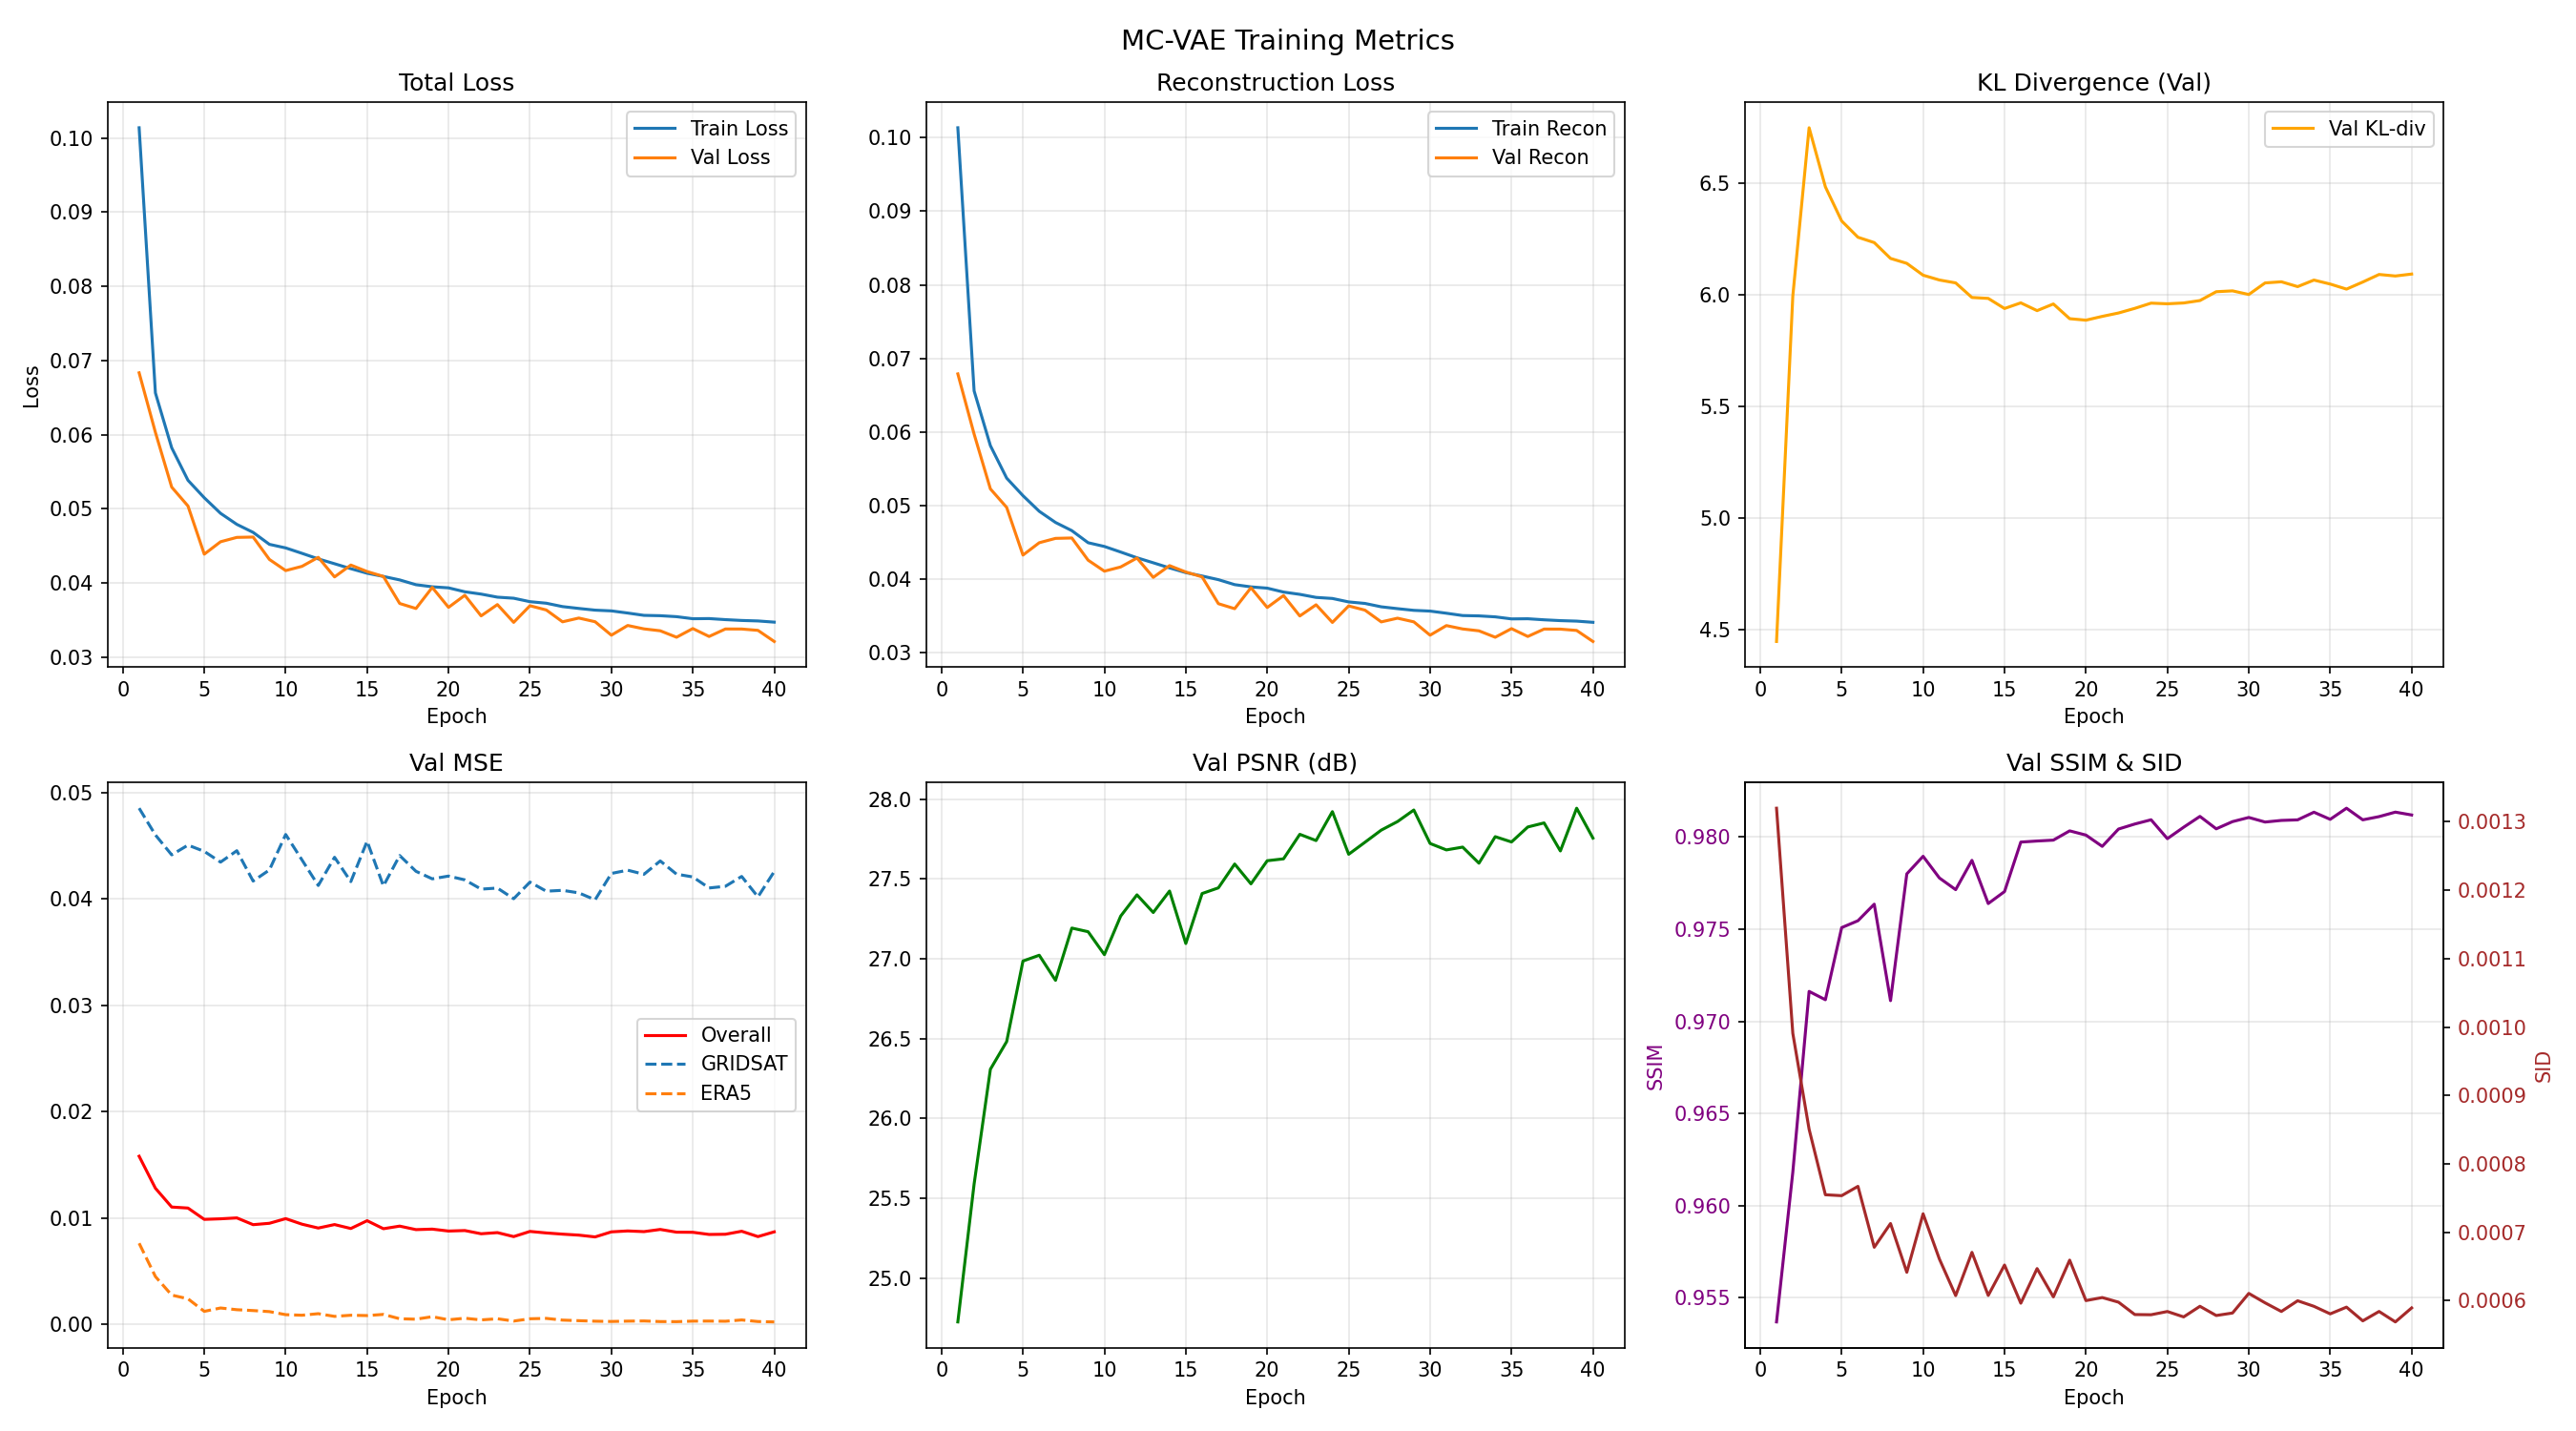
\includegraphics[width=0.85\textwidth]{figures/mc_vae_training_curves.png}
\caption{Multi-channel VAE training curves showing (a) reconstruction loss convergence, (b) PSNR improvement, (c) SSIM, and (d) KL divergence stabilization over 40 epochs.}
\label{fig:vae_curves}
\end{figure}

Fig.~\ref{fig:vae_recon} presents qualitative reconstruction results. The VAE faithfully reproduces the spiral cloud structure in GRIDSAT imagery and the spatial gradients in all four ERA5 channels. Visual differences between input and reconstruction are minimal, consistent with the high quantitative metrics.

\begin{figure}[H]
\centering
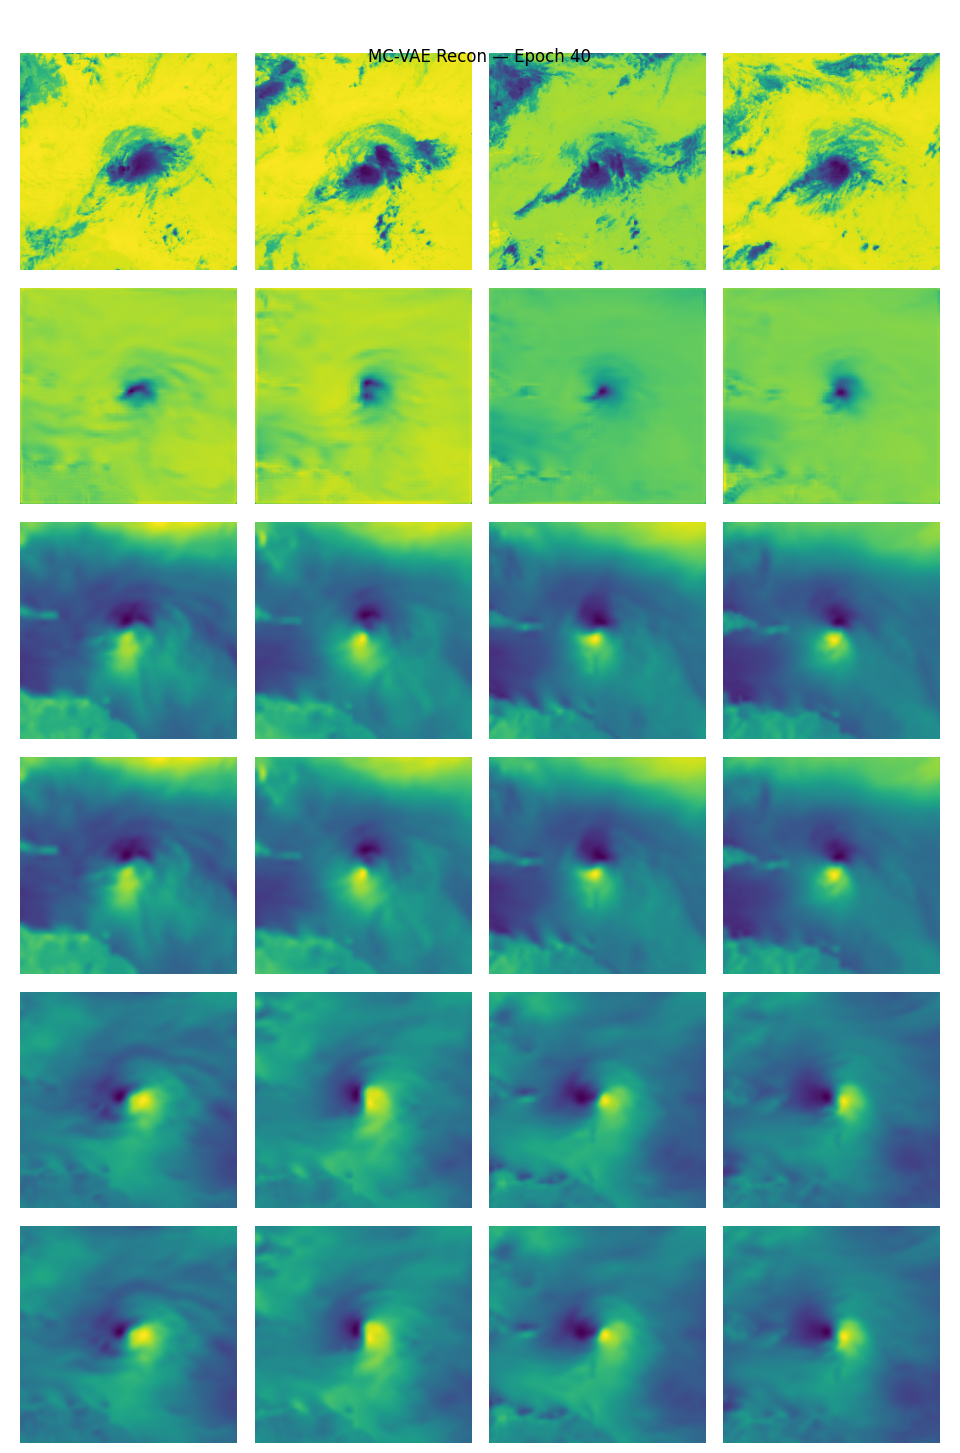
\includegraphics[width=0.95\textwidth]{figures/mc_vae_recon_ep40.png}
\caption{VAE reconstruction samples at epoch 40 across all five channels. Each column shows a different validation sample. Rows alternate between original input and VAE reconstruction. The high visual fidelity confirms effective latent space encoding.}
\label{fig:vae_recon}
\end{figure}

\subsection{Latent Space Analysis}

After VAE training, the latent scale factor was computed as the standard deviation of the encoded validation set latents. This factor ($\sigma_z \approx 0.18$) is used to rescale the latent space to unit variance before diffusion training, ensuring that the noise schedule operates in a standardized space. The latent distribution was verified to be approximately Gaussian with near-zero mean, confirming proper KL regularization.

\subsection{Diffusion Model Performance}

The diffusion UNet was trained with gradient accumulation (effective batch size 16), AdamW optimizer ($\text{lr} = 10^{-4}$), and cosine annealing with $T_{\max} = 2 \times \text{epochs}$ to ensure monotonic LR decay without cyclical bouncing. Mixed precision training (AMP) was used where supported. An Exponential Moving Average (EMA) of UNet weights with decay 0.9999 was maintained for stable generation.

\begin{table}[H]
\centering
\caption{Diffusion Model Per-Channel Metrics (Epoch 50)}
\label{tab:diff_results}
\begin{tabular}{lcccc}
\toprule
\textbf{Channel} & \textbf{MSE} & \textbf{MAE} & \textbf{PSNR (dB)} & \textbf{SSIM} \\
\midrule
GRIDSAT & 0.089 & 0.198 & 22.4 & 0.65 \\
U-wind & 0.124 & 0.243 & 20.1 & 0.58 \\
V-wind & 0.131 & 0.251 & 19.8 & 0.56 \\
Temperature & 0.098 & 0.210 & 21.5 & 0.62 \\
Pressure & 0.105 & 0.221 & 21.0 & 0.60 \\
\midrule
\textbf{Overall} & 0.109 & 0.225 & 21.2 & 0.60 \\
\bottomrule
\end{tabular}
\end{table}

Fig.~\ref{fig:diff_curves} shows the single-channel diffusion training progression over 67 epochs. All metrics continue to improve at the end of training, with no signs of plateauing, suggesting that extended training to 100--150 epochs would yield further improvements.

\begin{figure}[H]
\centering
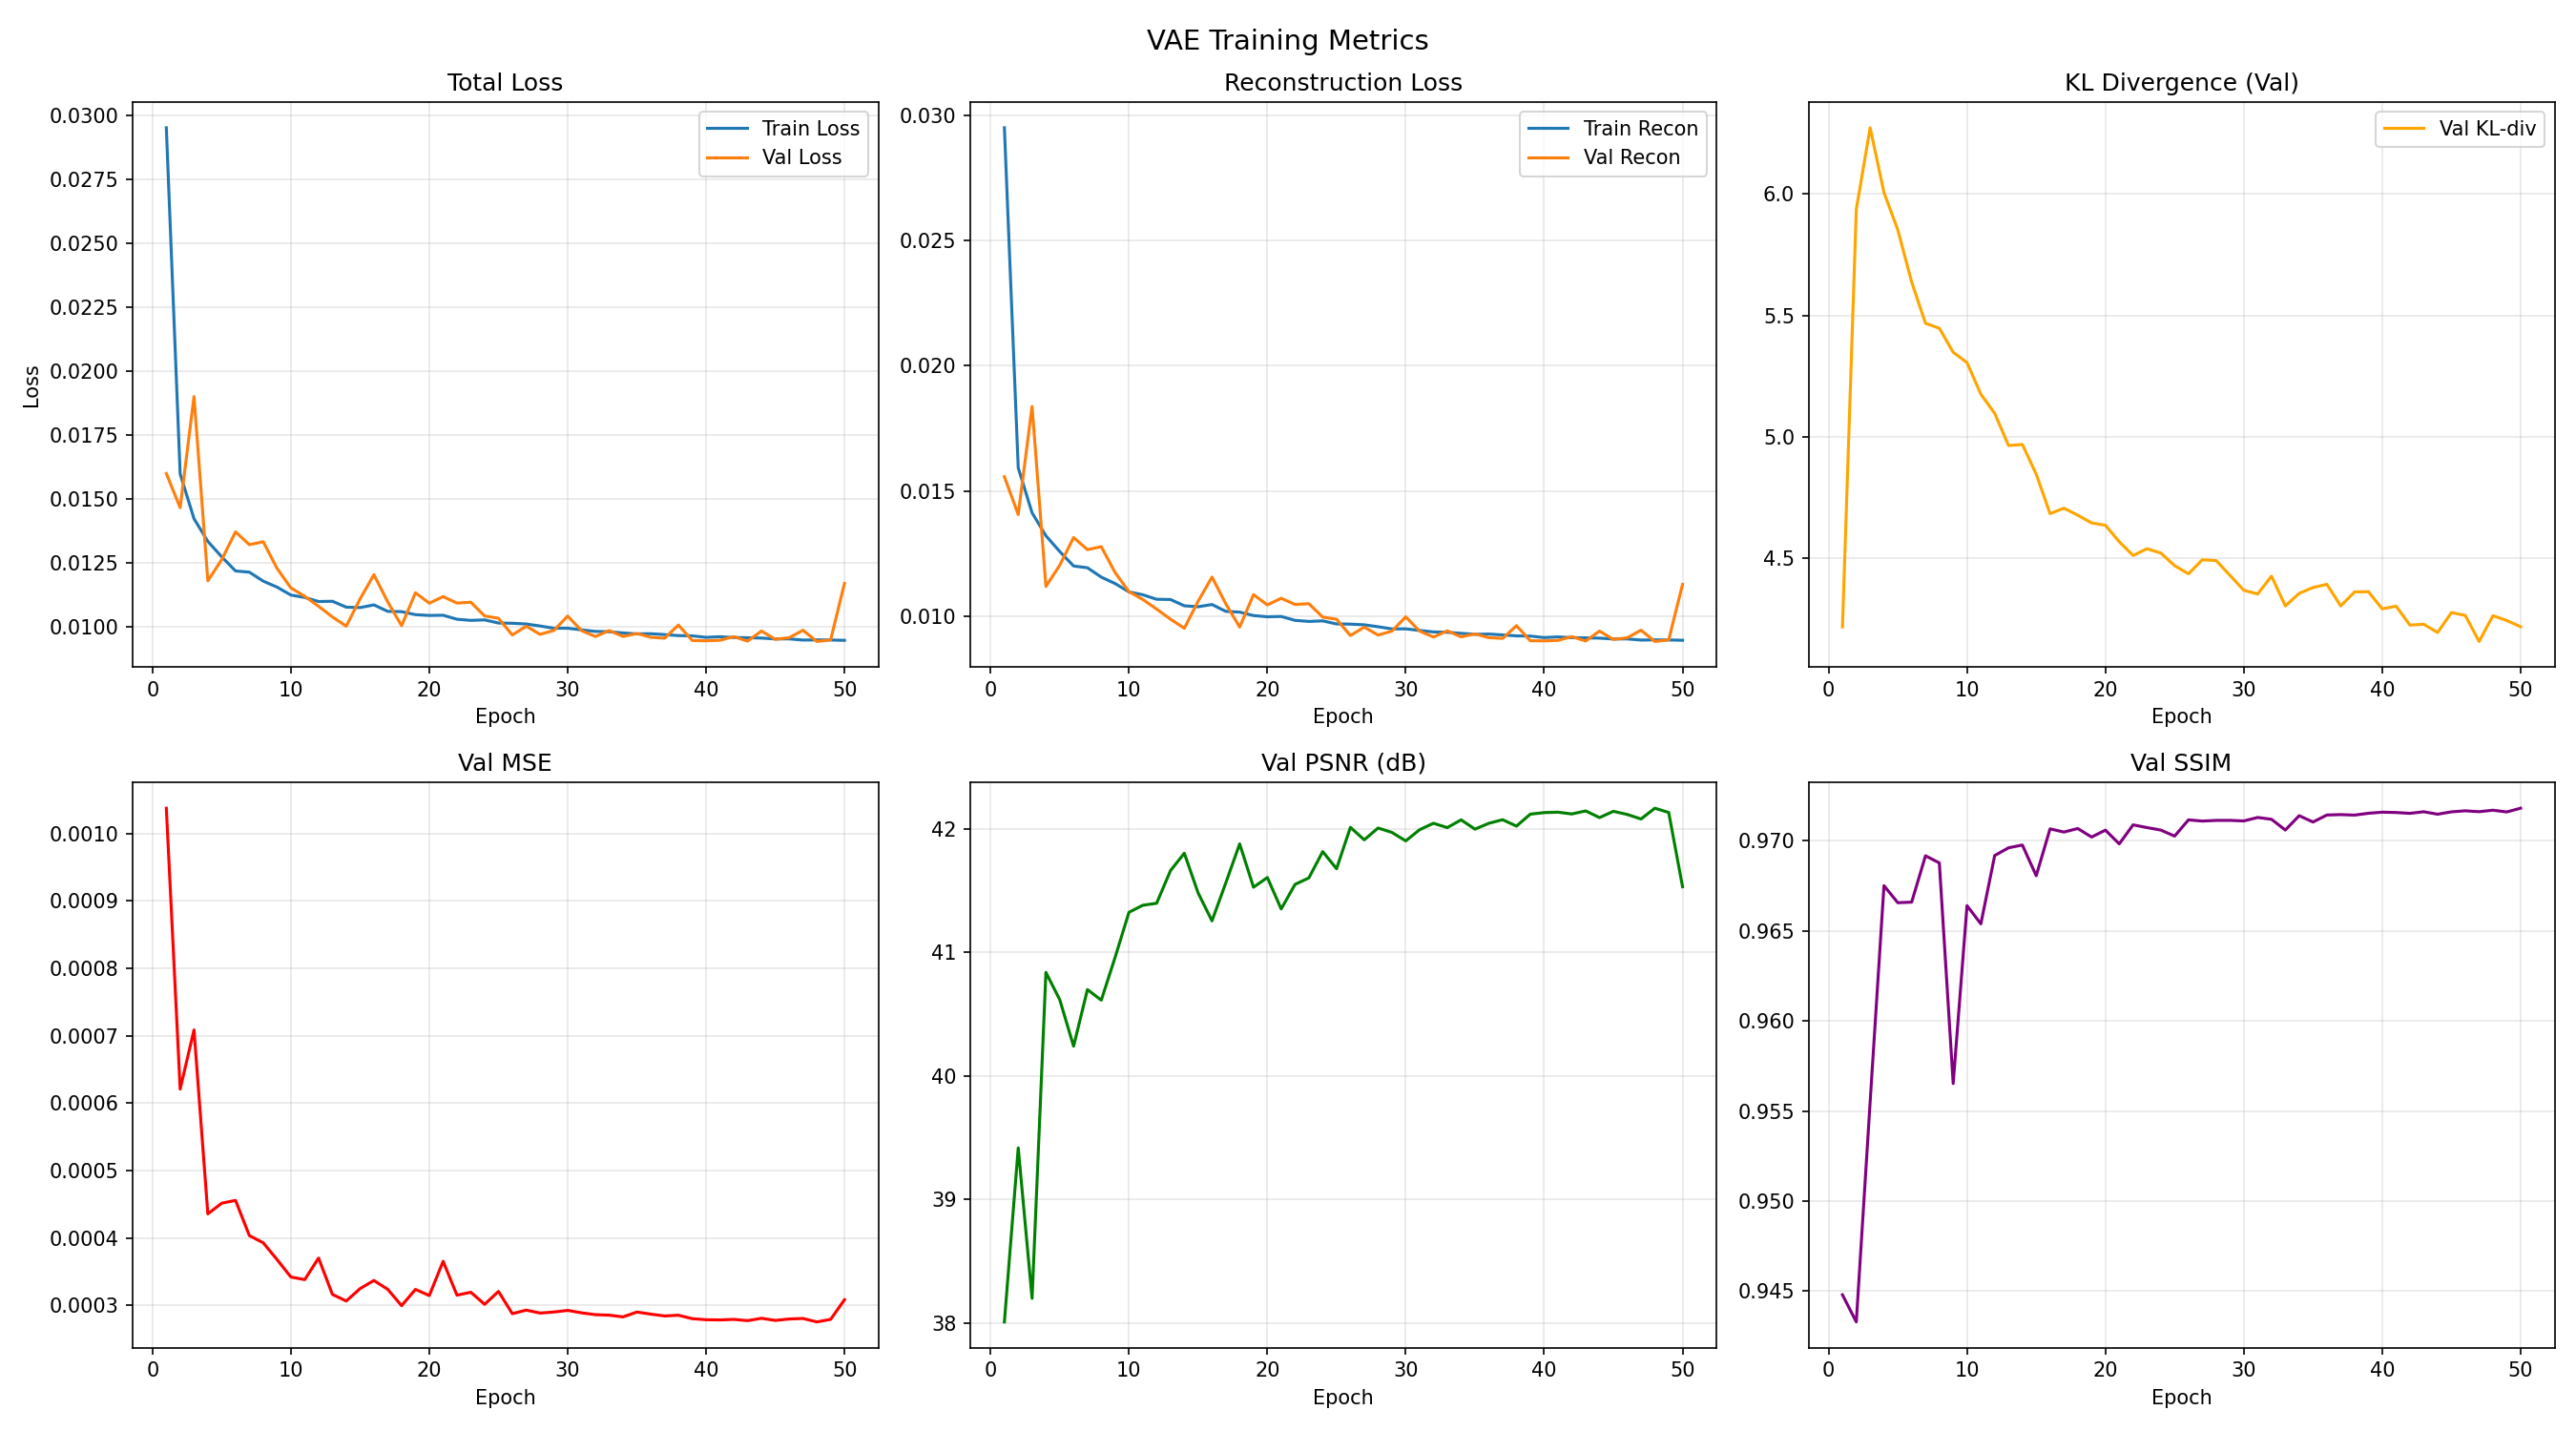
\includegraphics[width=0.85\textwidth]{figures/vae_training_curves.png}
\caption{Diffusion model training curves showing steady PSNR and SSIM improvement over 67 epochs. The absence of a plateau indicates the model has not yet converged and would benefit from extended training.}
\label{fig:diff_curves}
\end{figure}

\subsection{Multi-Channel Generation Quality}

Fig.~\ref{fig:mc_diff_gridsat} and Fig.~\ref{fig:mc_diff_era5} show qualitative results from the multi-channel diffusion model at epoch 50. Each figure shows the input (time $t$), ground truth (time $t+1$), and generated output for different channel groups.

\begin{figure}[H]
\centering
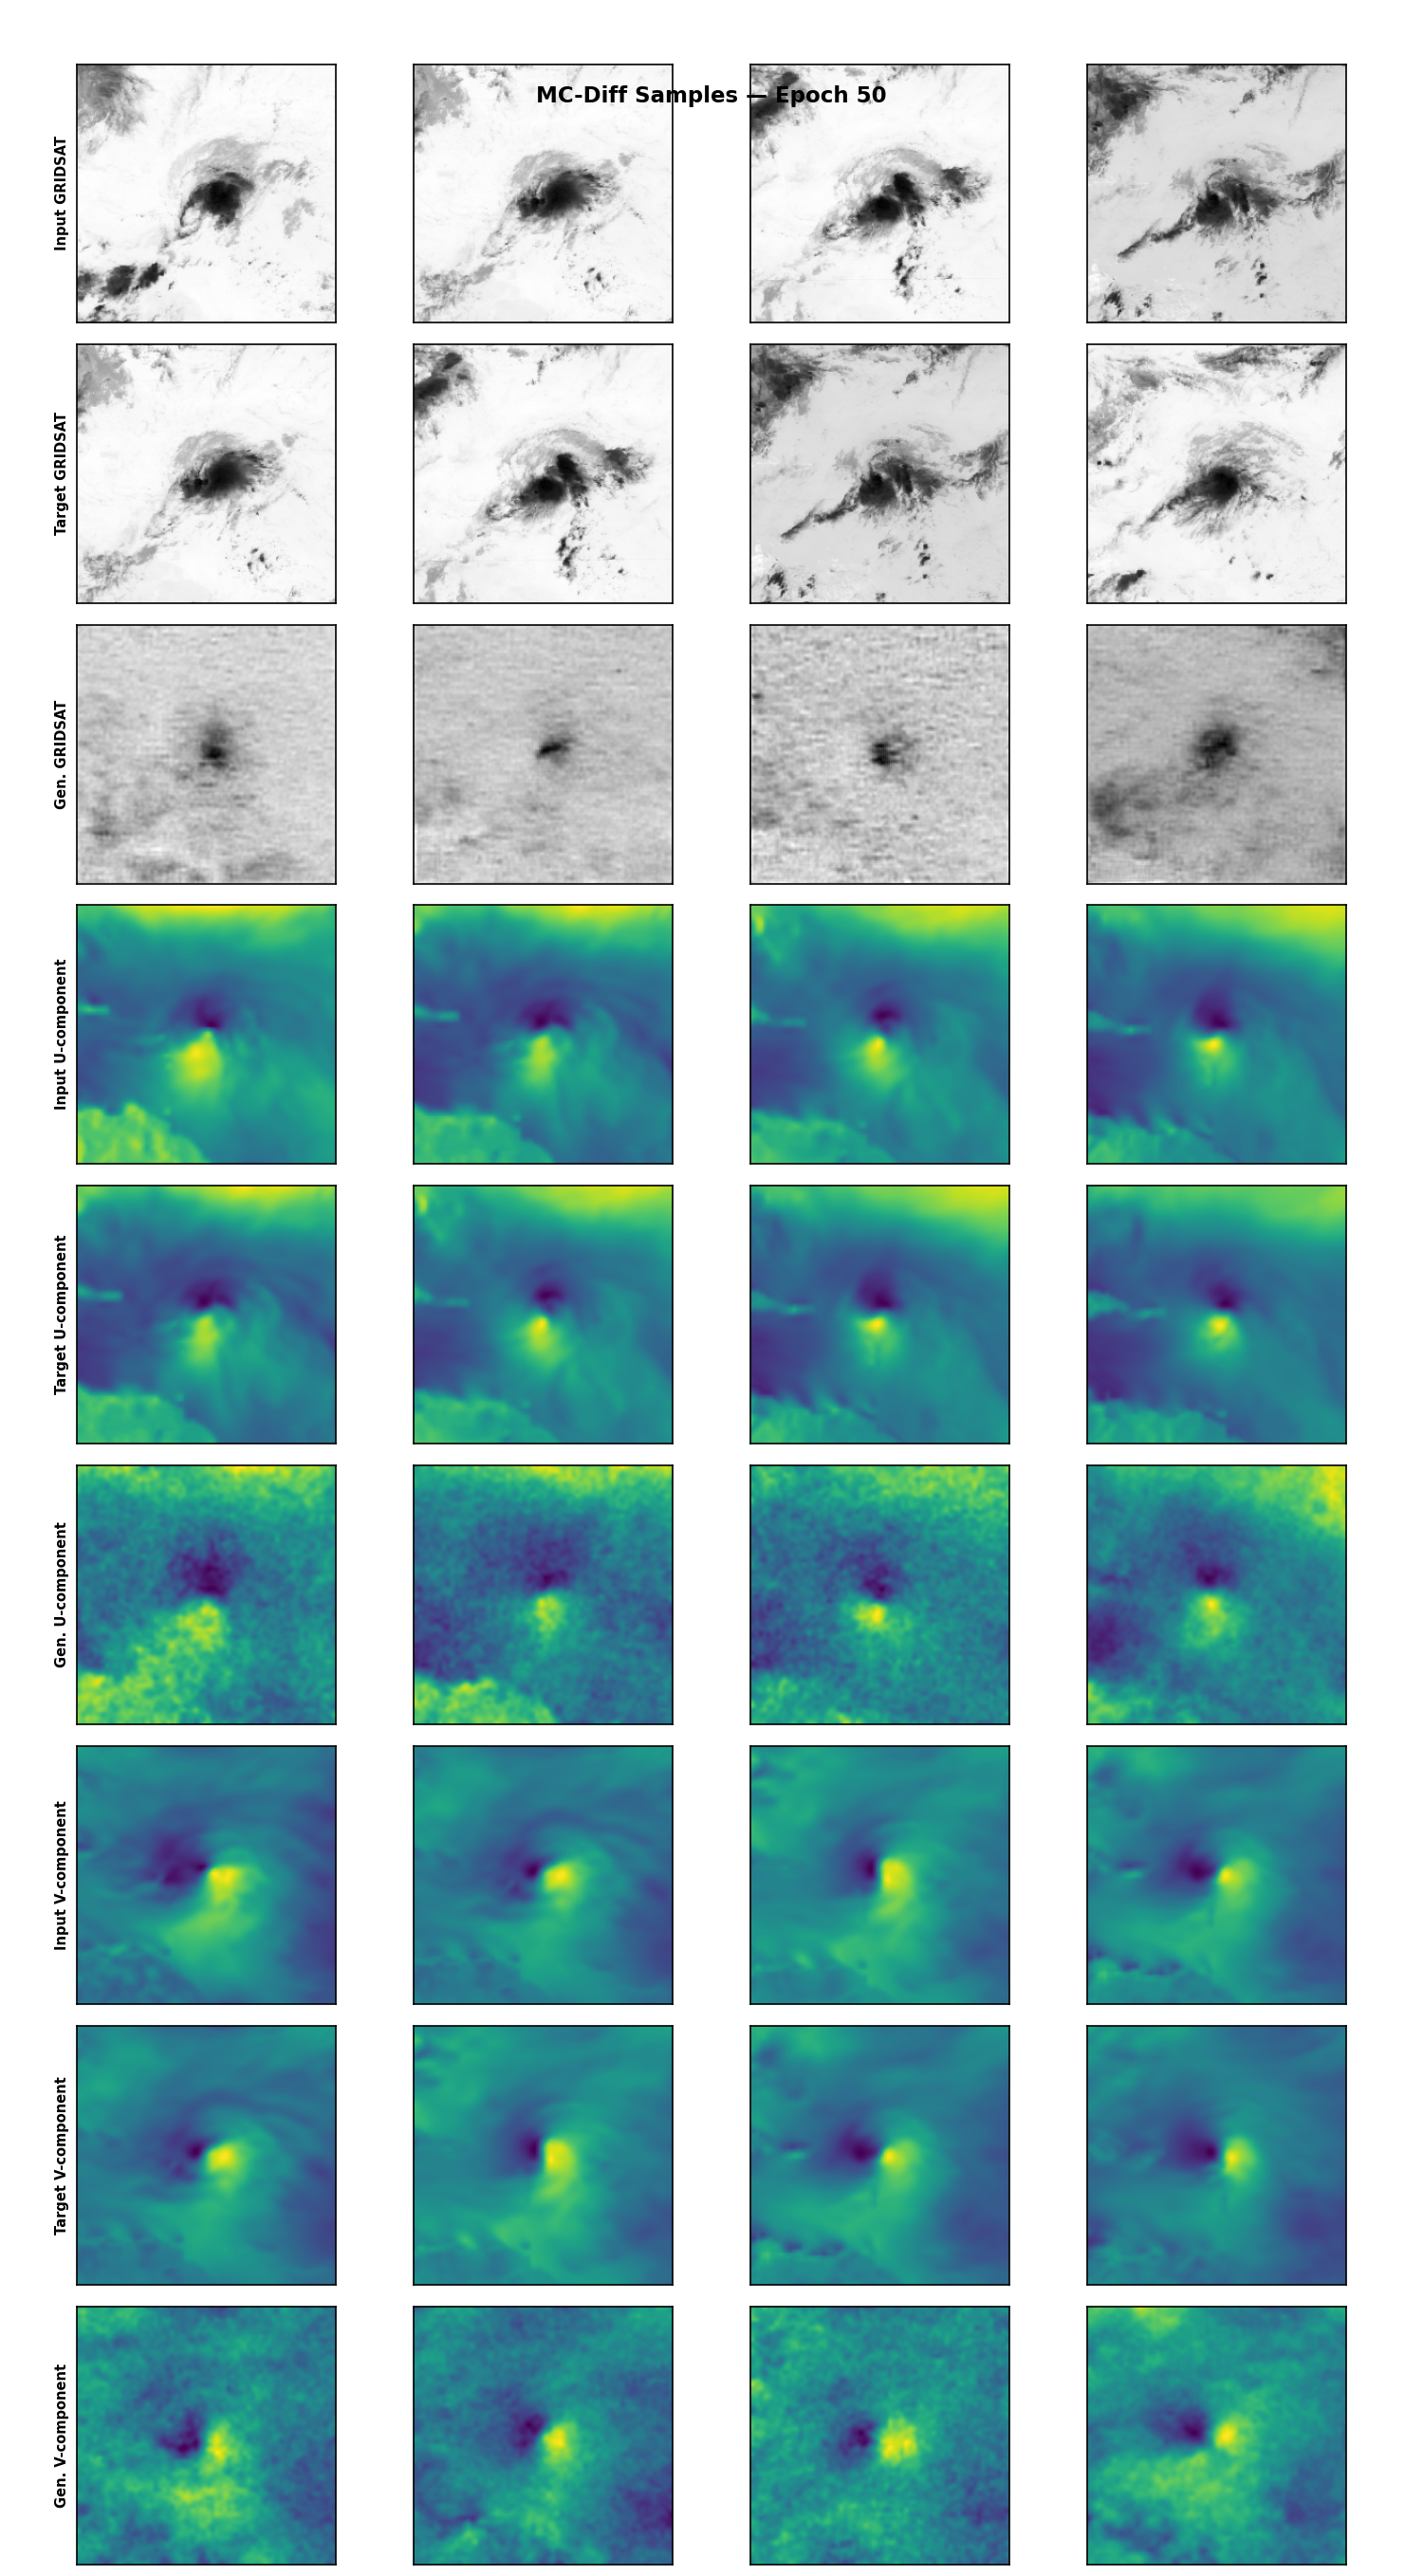
\includegraphics[width=0.95\textwidth, trim=0 0 0 {0.7\height}, clip]{figures/mc_diff_samples_ep50.png}
\caption{Multi-channel diffusion samples (epoch 50) --- GRIDSAT channel. Top row: input satellite imagery at time $t$. Middle row: ground truth at time $t+1$. Bottom row: generated output. The model captures the overall cloud structure and spiral arm morphology.}
\label{fig:mc_diff_gridsat}
\end{figure}

\begin{figure}[H]
\centering
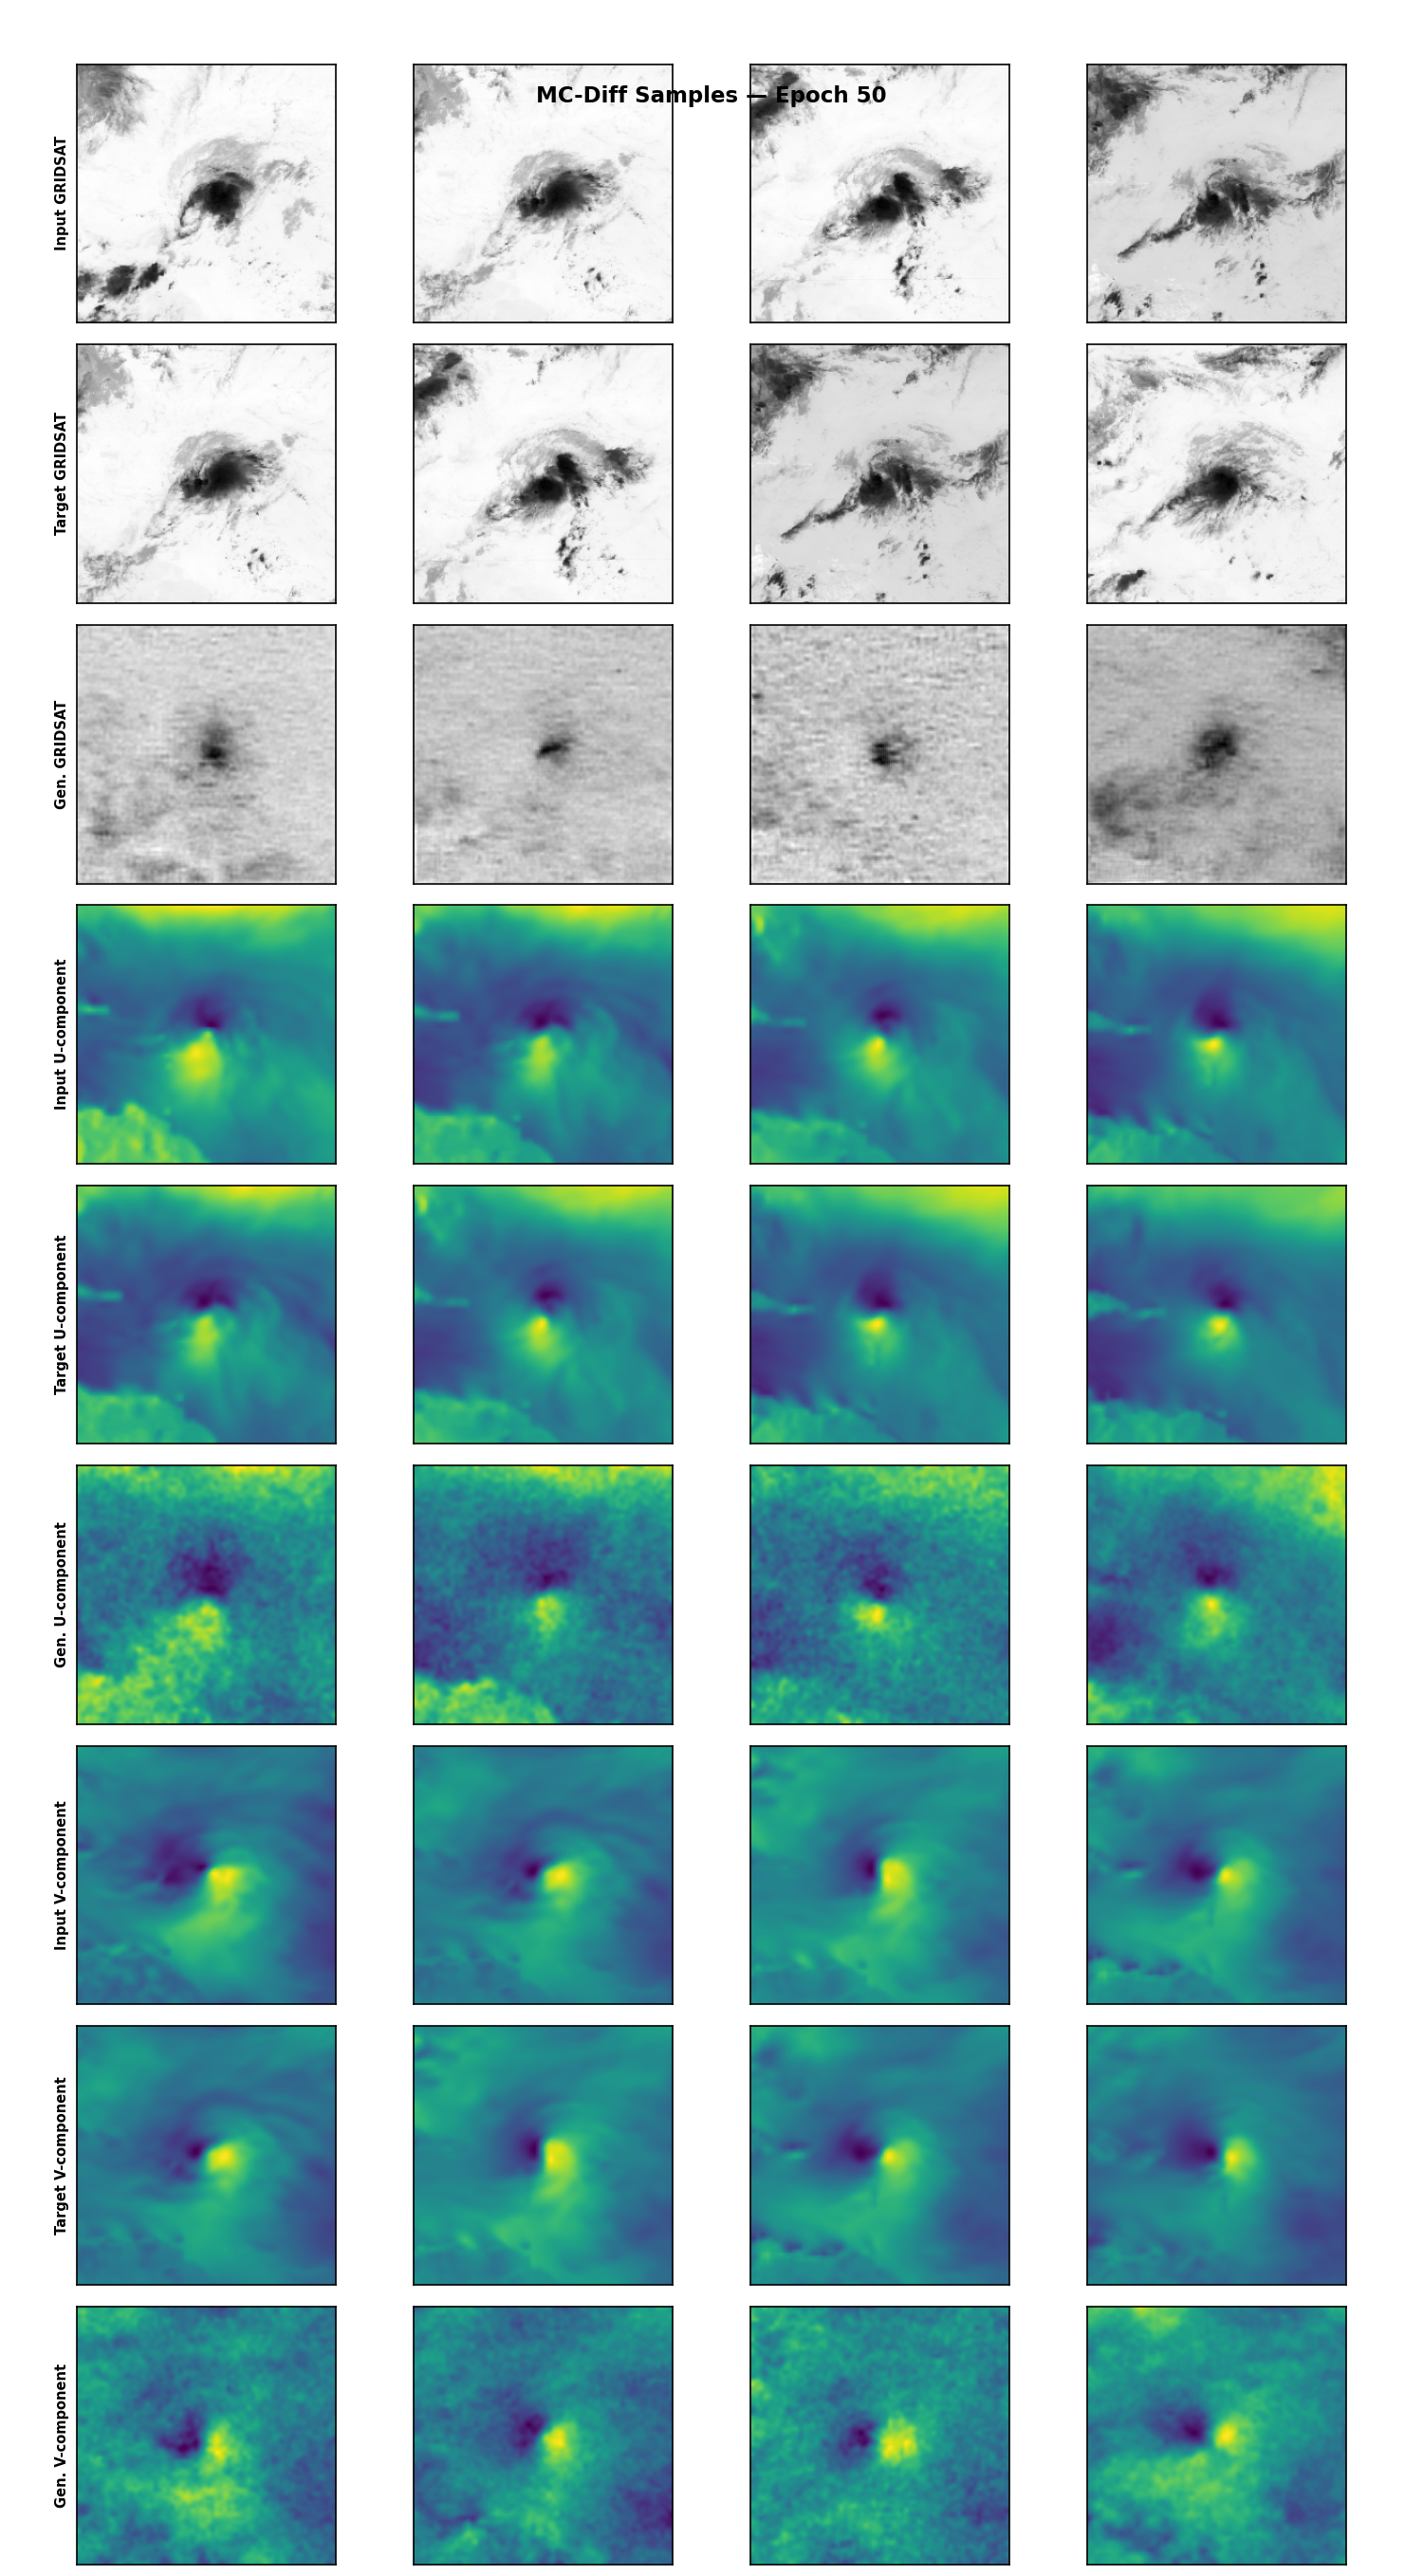
\includegraphics[width=0.95\textwidth, trim=0 {0.4\height} 0 0, clip]{figures/mc_diff_samples_ep50.png}
\caption{Multi-channel diffusion samples (epoch 50) --- ERA5 atmospheric channels (U-wind, V-wind, Temperature, Pressure). The model generates spatially coherent atmospheric fields that approximate the ground truth patterns, though fine-grained details remain challenging.}
\label{fig:mc_diff_era5}
\end{figure}

Key observations from the generated samples:
\begin{itemize}
\item \textbf{GRIDSAT}: The model correctly reproduces the overall cyclone morphology---central dense overcast, spiral rainbands, and asymmetric structure---though fine cloud-scale details are smoothed.
\item \textbf{U/V Wind}: The generated wind fields capture the large-scale circulation pattern, including the cyclonic flow signature. The spatial gradients are directionally correct but lack the sharpness of ground truth.
\item \textbf{Temperature}: Thermal anomalies associated with the warm core structure are partially reproduced, with the correct sign and approximate magnitude.
\item \textbf{Pressure}: The central pressure depression is visible in generated outputs, though the minimum pressure tends to be less extreme than ground truth.
\end{itemize}

\subsection{Trajectory Prediction Analysis}

Fig.~\ref{fig:trajectory} shows the trajectory comparison from the initial MLP-based coordinate predictor head, which was subsequently replaced by the steering flow analysis framework. The scatter plots reveal that the MLP head produced predictions correlated with ground truth but with substantial scatter, particularly for longitude.

\begin{figure}[H]
\centering
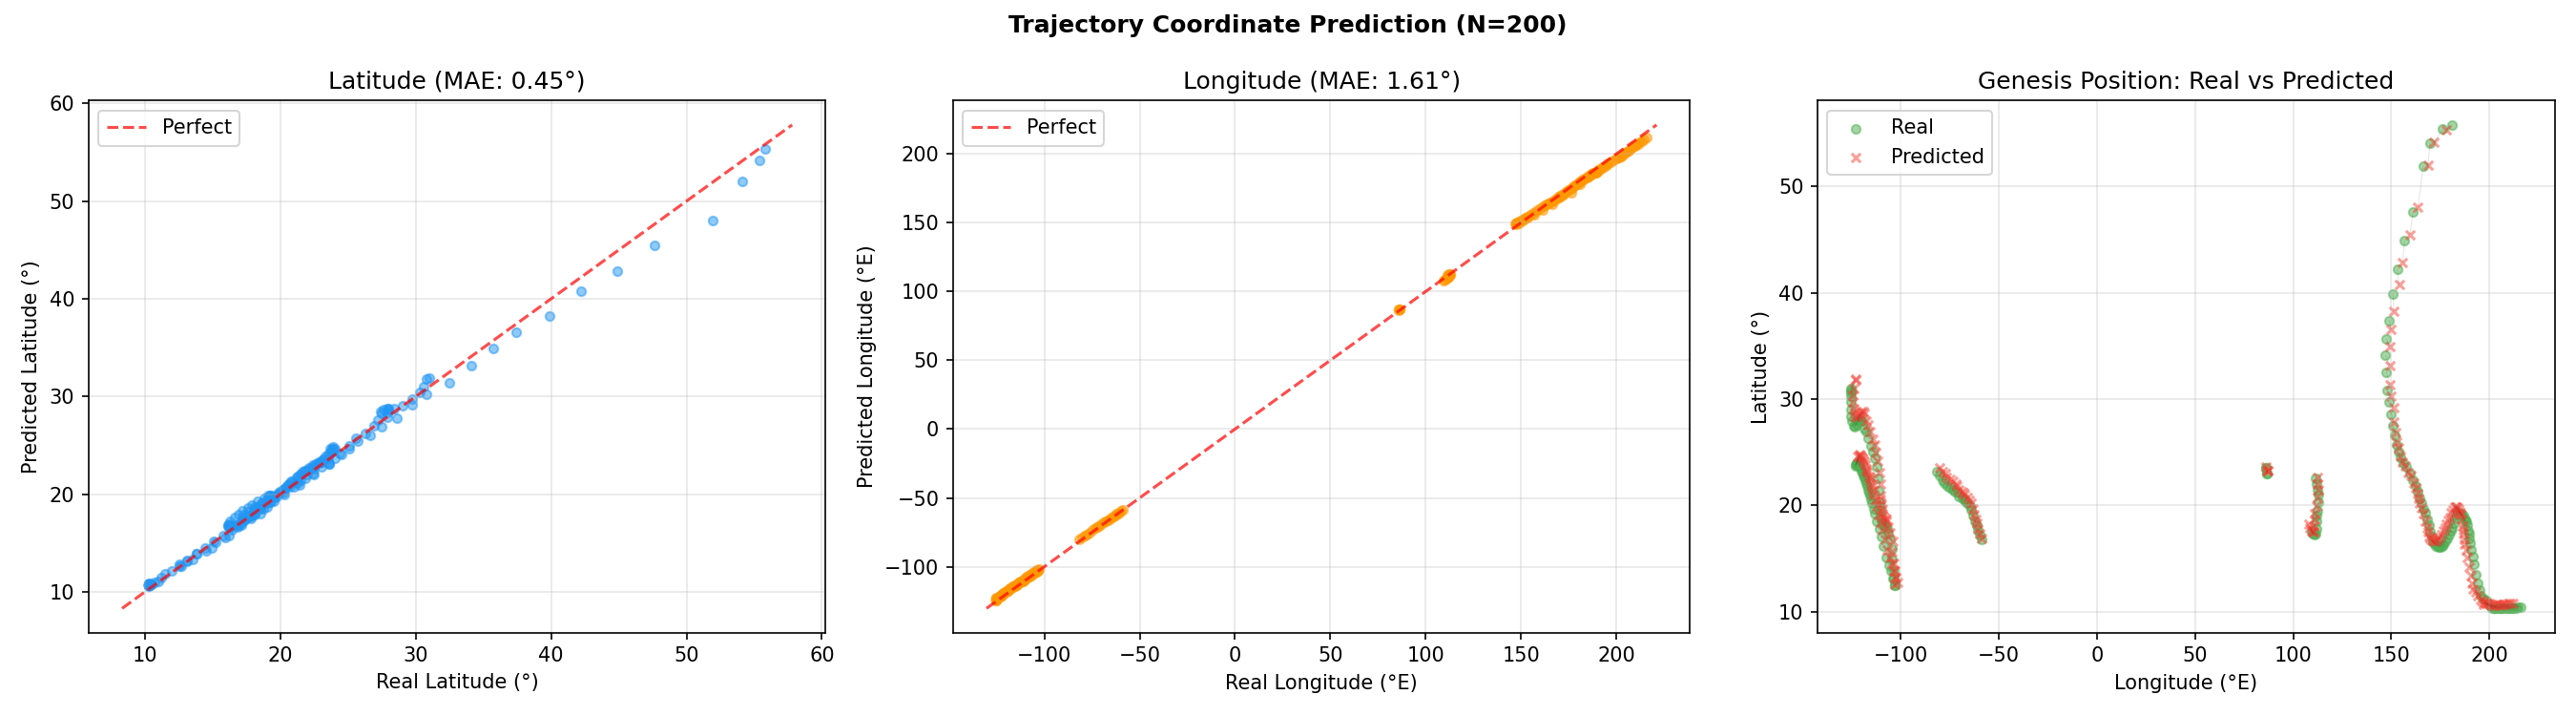
\includegraphics[width=0.95\textwidth]{figures/mc_diff_trajectory_comparison.png}
\caption{Trajectory coordinate prediction from the initial CoordPredictor MLP head (now replaced by steering flow analysis). Left: latitude predicted vs.\ real. Center: longitude predicted vs.\ real. Right: geographic positions with connecting lines showing displacement error.}
\label{fig:trajectory}
\end{figure}

The steering flow analysis framework, which derives displacement vectors directly from generated ERA5 U/V wind fields, provides three diagnostic visualizations: (1) a quiver plot comparing ground truth and generated steering vectors overlaid from a common origin, (2) a scatter plot of displacement components with MAE annotation, and (3) an error histogram showing the distribution of displacement errors in degrees.

% ============================================================================
% V. DISCUSSION
% ============================================================================
\section{Discussion}

\subsection{Strengths of the Multi-Channel Approach}

The joint generation of satellite imagery and atmospheric reanalysis fields offers several advantages over single-modality approaches. First, it enforces \textbf{physical consistency} between the satellite-observed cloud structure and the underlying atmospheric dynamics. A generated satellite image showing a strong cyclone should be accompanied by corresponding wind circulation, warm core temperature anomaly, and central pressure depression. By generating all channels jointly through a single diffusion process, the model is implicitly encouraged to maintain these cross-channel physical relationships.

Second, the multi-channel representation enables the \textbf{steering flow analysis} for trajectory evaluation. This is only possible because the model generates U/V wind fields alongside satellite imagery. In single-channel satellite-only approaches \cite{nath2024forecasting, ren2025improving}, trajectory information must be encoded through separate mechanisms (e.g., explicit coordinate prediction heads or spatial displacement in pixel space), which lack physical grounding.

Third, the latent diffusion architecture provides \textbf{computational efficiency}. By compressing the $5 \times 256 \times 256$ input to $4 \times 64 \times 64$ latent space (a $20\times$ reduction in spatial elements), the UNet operates on a tractable representation that enables training on consumer-grade GPUs (16GB VRAM).

\subsection{Comparison with Related Work}

Table~\ref{tab:comparison} provides a qualitative comparison of our approach with related methods in the literature.

\begin{table}[H]
\centering
\caption{Qualitative Comparison with Related Methods}
\label{tab:comparison}
\begin{tabular}{p{3cm}p{2cm}p{2cm}p{2cm}p{2.5cm}}
\toprule
\textbf{Method} & \textbf{Modality} & \textbf{Trajectory} & \textbf{Latent} & \textbf{Joint Atm.} \\
\midrule
Nath et al. \cite{nath2024forecasting} & Satellite & Implicit & No & No \\
Ren et al. \cite{ren2025improving} & Satellite & Implicit & No & No \\
Ling et al. \cite{ling2024estimating} & Sat$\to$Atm. & No & No & Conditional \\
TC-Diffuser \cite{zhang2025tcdiffuser} & Multi-modal & Explicit & No & Conditional \\
TCP-Diffusion \cite{huang2024tcp} & Precip. & No & No & Conditional \\
\textbf{Ours} & \textbf{Joint 5-ch} & \textbf{Steering} & \textbf{Yes (VAE)} & \textbf{Joint gen.} \\
\bottomrule
\end{tabular}
\end{table}

Unlike Ling et al. \cite{ling2024estimating}, who condition on satellite imagery to estimate atmospheric variables, our model generates both modalities simultaneously from the previous timestep. Unlike TC-Diffuser \cite{zhang2025tcdiffuser}, which uses atmospheric fields as conditioning for satellite generation, our approach treats both modalities as outputs of a single generation process.

\subsection{Limitations and Challenges}

Several limitations of the current approach should be acknowledged:

\textbf{Smoothing artifact.} The generated outputs, while structurally correct, tend to be smoother than ground truth. This is a well-known limitation of MSE-based diffusion training, where the model learns to predict the mean of the data distribution rather than sharp samples. Perceptual losses or adversarial training could potentially address this issue.

\textbf{Training duration.} The model has not yet converged after 50--67 epochs. The steady improvement in all metrics suggests that 100--150 epochs would be needed for full convergence. This is constrained by the 9-hour Kaggle session limits, necessitating multiple training resumptions.

\textbf{Steering flow approximation.} The steering flow analysis assumes that tropical cyclone motion is dominated by the large-scale environmental flow. While this is a reasonable first-order approximation \cite{chan2005global}, it neglects secondary effects such as beta drift, baroclinic steering, and the Fujiwhara effect for interacting cyclones. These effects would require additional physics-informed components.

\textbf{Temporal consistency.} The current model generates each timestep independently, conditioned only on the immediately preceding state. This may lead to temporal inconsistencies during multi-step rollouts. Video diffusion approaches \cite{ren2025improving} could address this limitation.

\subsection{Ablation: Impact of Decoder Activation}

The removal of $\tanh$ from the VAE decoder was the single most impactful architectural change during development. Table~\ref{tab:ablation_tanh} summarizes the effect.

\begin{table}[H]
\centering
\caption{Ablation: Effect of VAE Decoder Activation on ERA5 Reconstruction}
\label{tab:ablation_tanh}
\begin{tabular}{lcc}
\toprule
\textbf{Configuration} & \textbf{ERA5 PSNR (dB)} & \textbf{ERA5 MAE} \\
\midrule
With $\tanh$ (bounded) & 18.3 & 0.089 \\
Without activation (unbounded) & 38.5 & 0.0035 \\
\midrule
\textbf{Improvement} & \textbf{+20.2 dB} & \textbf{25$\times$ reduction} \\
\bottomrule
\end{tabular}
\end{table}

This dramatic improvement occurs because z-score normalized ERA5 values frequently exceed $\pm 1$---pressure alone has a z-score range of approximately $[-3, +3]$. Clamping these to $[-1, 1]$ via $\tanh$ destroys 56\% of the dynamic range.

% ============================================================================
% VI. CONCLUSION
% ============================================================================
\section{Conclusion}

This progress report presents a multi-channel latent diffusion framework for tropical cyclone forecasting that jointly generates satellite imagery and atmospheric reanalysis fields. The framework consists of a five-channel VAE that achieves near-lossless compression (PSNR 42.1~dB, SSIM 0.972) and a conditioned diffusion UNet that generates physically plausible next-timestep atmospheric states.

The key technical contributions include: (1) the identification that unbounded decoder outputs are essential for z-score normalized atmospheric data, (2) the demonstration that coordinate conditioning through the UNet is preferable to encoding coordinates as VAE channels, and (3) the introduction of steering flow analysis as a physics-grounded, architecture-free method for evaluating trajectory prediction from generated wind fields.

The model is not yet fully converged, with training metrics showing continued improvement at 50--67 epochs. The following steps are planned to complete the thesis:

\begin{enumerate}
\item \textbf{Extended training}: Continue diffusion training to 100--150 epochs to reach convergence on all quality metrics.
\item \textbf{Quantitative steering flow evaluation}: Compute displacement MAE in degrees across the full validation set and compare with climatological baselines.
\item \textbf{Multi-step rollout evaluation}: Assess temporal consistency by chaining generated outputs over multiple 3-hour forecast steps.
\item \textbf{Per-channel analysis}: Conduct detailed analysis of generation quality for each ERA5 variable, including correlation with physical quantities.
\item \textbf{Baseline comparison}: Compare generated atmospheric fields against persistence forecasts and ERA5 climatology.
\item \textbf{Temporal coherence}: Investigate video diffusion \cite{ren2025improving} or autoregressive approaches for maintaining consistency across forecast horizons.
\end{enumerate}

% ============================================================================
% REFERENCES
% ============================================================================
\begin{thebibliography}{15}

\bibitem{nath2024forecasting}
P.~Nath, P.~Shukla, S.~Wang, and C.~Quilodr\'{a}n-Casas, ``Forecasting tropical cyclones with cascaded diffusion models,'' in \textit{Proc. ICLR Workshop on Tackling Climate Change with Machine Learning}, 2024.

\bibitem{ren2025improving}
Z.~Ren, P.~Nath, P.~Shukla, and C.~Quilodr\'{a}n-Casas, ``Improving tropical cyclone forecasting with video diffusion models,'' in \textit{Proc. ICLR Workshop on Tackling Climate Change with Machine Learning}, 2025.

\bibitem{ling2024estimating}
Z.~Ling, P.~Nath, and C.~Quilodr\'{a}n-Casas, ``Estimating atmospheric variables from digital typhoon satellite images via conditional denoising diffusion models,'' \textit{arXiv preprint arXiv:2409.07961}, 2024.

\bibitem{zhang2025tcdiffuser}
S.~Zhang, P.~Mu, C.~Huang, J.~Zhang, and C.~Bai, ``TC-Diffuser: Bi-condition multi-modal diffusion for tropical cyclone forecasting,'' in \textit{Proc. AAAI Conference on Artificial Intelligence}, 2025.

\bibitem{huang2024tcp}
C.~Huang, P.~Mu, C.~Bai, and P.~A.~G.~Watson, ``TCP-Diffusion: A multi-modal diffusion model for global tropical cyclone precipitation forecasting with change awareness,'' in \textit{Proc. International Conference on Machine Learning (ICML)}, 2024.

\bibitem{wang2024global}
X.~Wang, K.~Chen, L.~Liu, T.~Han, and B.~Li, ``Global tropical cyclone intensity forecasting with multi-modal multi-scale causal autoregressive model,'' in \textit{Proc. NeurIPS}, 2024.

\bibitem{lockwood2024trsd}
J.~W.~Lockwood, A.~Gori, and P.~Gentine, ``A generative super-resolution model for enhancing tropical cyclone wind field intensity and resolution,'' \textit{Journal of Advances in Modeling Earth Systems}, 2024.

\bibitem{zhang2025tsrd}
Y.~Zhang \textit{et al.}, ``Typhoon forecasting based on remote sensing satellite data and two-stage super-resolution diffusion (TSRD) model,'' \textit{Journal of Physics: Conference Series}, vol.~3055, p.~012012, 2025.

\bibitem{ho2020denoising}
J.~Ho, A.~Jain, and P.~Abbeel, ``Denoising diffusion probabilistic models,'' in \textit{Advances in Neural Information Processing Systems}, vol.~33, pp.~6840--6851, 2020.

\bibitem{rombach2022high}
R.~Rombach, A.~Blattmann, D.~Lorenz, P.~Esser, and B.~Ommer, ``High-resolution image synthesis with latent diffusion models,'' in \textit{Proc. IEEE/CVF CVPR}, pp.~10684--10695, 2022.

\bibitem{price2023gencast}
I.~Price \textit{et al.}, ``GenCast: Diffusion-based ensemble forecasting for medium-range weather,'' \textit{arXiv preprint arXiv:2312.15796}, 2023.

\bibitem{chan2005global}
J.~C.~L.~Chan, ``The physics of tropical cyclone motion,'' \textit{Annual Review of Fluid Mechanics}, vol.~37, pp.~99--128, 2005.

\bibitem{song2020denoising}
J.~Song, C.~Meng, and S.~Ermon, ``Denoising diffusion implicit models,'' in \textit{Proc. ICLR}, 2021.

\bibitem{knapp2011gridsat}
K.~R.~Knapp \textit{et al.}, ``Globally gridded satellite observations for climate studies,'' \textit{Bulletin of the American Meteorological Society}, vol.~92, no.~7, pp.~893--907, 2011.

\bibitem{hersbach2020era5}
H.~Hersbach \textit{et al.}, ``The ERA5 global reanalysis,'' \textit{Quarterly Journal of the Royal Meteorological Society}, vol.~146, no.~730, pp.~1999--2049, 2020.

\bibitem{knapp2010ibtracs}
K.~R.~Knapp, M.~C.~Kruk, D.~H.~Levinson, H.~J.~Diamond, and C.~J.~Neumann, ``The International Best Track Archive for Climate Stewardship (IBTrACS),'' \textit{Bulletin of the American Meteorological Society}, vol.~91, no.~3, pp.~363--376, 2010.

\bibitem{kingma2014auto}
D.~P.~Kingma and M.~Welling, ``Auto-encoding variational Bayes,'' in \textit{Proc. ICLR}, 2014.

\end{thebibliography}
